\title{Report for summer school CPS2018}
\author{
        \textsc{Lingyuan Yang}
            \qquad
        \\
        \normalsize
            \texttt{linyan@kth.se}
}
\date{\today}

\documentclass[12pt,twoside]{article}

\usepackage[paper=a4paper,dvips,top=1.5cm,left=1.5cm,right=1.5cm,
    foot=1cm,bottom=1.5cm]{geometry}


%\usepackage[T1]{fontenc}
%%\usepackage{pslatex}
\renewcommand{\rmdefault}{ptm} 
\usepackage{mathptmx}
\usepackage{amsmath}
\usepackage[scaled=.90]{helvet}
\usepackage{courier}

\usepackage[center]{titlesec}
\usepackage{bookmark}

\usepackage{fancyhdr}
\pagestyle{fancy}

%%----------------------------------------------------------------------------
%%   pcap2tex stuff
%%----------------------------------------------------------------------------
 \usepackage[dvipsnames*,svgnames]{xcolor} %% For extended colors
 \usepackage{tikz}
 \usetikzlibrary{arrows,decorations.pathmorphing,backgrounds,fit,positioning,calc,shapes}

%% \usepackage{pgfmath}	% --math engine
%%----------------------------------------------------------------------------
%% \usepackage[latin1]{inputenc}
\usepackage[utf8]{inputenc} % inputenc allows the user to input accented characters directly from the keyboard
\usepackage[english]{babel}
%% \usepackage{rotating}		 %% For text rotating
\usepackage{array}			 %% For table wrapping
\usepackage{graphicx}	                 %% Support for images
\usepackage{float}			 %% Suppor for more flexible floating box positioning
\usepackage{color}                       %% Support for colour 
\usepackage{mdwlist}
%% \usepackage{setspace}                 %% For fine-grained control over line spacing
%% \usepackage{listings}		 %% For source code listing
%% \usepackage{bytefield}                %% For packet drawings
\usepackage{tabularx}		         %% For simple table stretching
%%\usepackage{multirow}	                 %% Support for multirow colums in tables
\usepackage{dcolumn}	                 %% Support for decimal point alignment in tables
\usepackage{url}	                 %% Support for breaking URLs
\usepackage[perpage,para,symbol]{footmisc} %% use symbols to ``number'' footnotes and reset which symbol is used first on each page

%% \usepackage{pygmentize}           %% required to use minted -- see python-pygments - Pygments is a Syntax Highlighting Package written in Python
%% \usepackage{minted}		     %% For source code highlighting

 \usepackage{hyperref}		
\usepackage[all]{hypcap}	 %% Prevents an issue related to hyperref and caption linking
%% setup hyperref to use the darkblue color on links
 \hypersetup{colorlinks,breaklinks,
             linkcolor=darkblue,urlcolor=darkblue,
             anchorcolor=darkblue,citecolor=darkblue}

%% Some definitions of used colors
\definecolor{darkblue}{rgb}{0.0,0.0,0.3} %% define a color called darkblue
\definecolor{darkred}{rgb}{0.4,0.0,0.0}
\definecolor{red}{rgb}{0.7,0.0,0.0}
\definecolor{lightgrey}{rgb}{0.8,0.8,0.8} 
\definecolor{grey}{rgb}{0.6,0.6,0.6}
\definecolor{darkgrey}{rgb}{0.4,0.4,0.4}
%% Reduce hyphenation as much as possible
\hyphenpenalty=15000 
\tolerance=1000

%% useful redefinitions to use with tables
\newcommand{\rr}{\raggedright} %% raggedright command redefinition
\newcommand{\rl}{\raggedleft} %% raggedleft command redefinition
\newcommand{\tn}{\tabularnewline} %% tabularnewline command redefinition

%% definition of new command for bytefield package
\newcommand{\colorbitbox}[3]{%
	\rlap{\bitbox{#2}{\color{#1}\rule{\width}{\height}}}%
	\bitbox{#2}{#3}}

%% command to ease switching to red color text
\newcommand{\red}{\color{red}}
%%redefinition of paragraph command to insert a breakline after it
\makeatletter
\renewcommand\paragraph{\@startsection{paragraph}{4}{\z@}%
  {-3.25ex\@plus -1ex \@minus -.2ex}%
  {1.5ex \@plus .2ex}%
  {\normalfont\normalsize\bfseries}}
\makeatother

%%redefinition of subparagraph command to insert a breakline after it
\makeatletter
\renewcommand\subparagraph{\@startsection{subparagraph}{5}{\z@}%
  {-3.25ex\@plus -1ex \@minus -.2ex}%
  {1.5ex \@plus .2ex}%
  {\normalfont\normalsize\bfseries}}
\makeatother

\setcounter{tocdepth}{3}	%% 3 depth levels in TOC
\setcounter{secnumdepth}{5}
%%%%%%%%%%%%%%%%%%%%%%%%%%%%%%%%%%%%%%%%%%%%%%%%%%%%%%%%%%%%%%%%%%%%
%% End of preamble
%%%%%%%%%%%%%%%%%%%%%%%%%%%%%%%%%%%%%%%%%%%%%%%%%%%%%%%%%%%%%%%%%%%%

\renewcommand{\headrulewidth}{0pt}
\lhead{CPS2018}
%% or \lhead{II2202, Fall 2016, Period 1}
\chead{Final project report}
\rhead{\date{\today}}

\makeatletter
\let\ps@plain\ps@fancy 
\makeatother

\setlength{\headheight}{15pt}
\begin{document}

\maketitle

\centering
\section*{Executive summary}

This report is for the cyber security and privacy summer school 2018 in Trento. The name of our project
is EspioNo. We provide device to secure your private conversation from listening by smart speakers.
With a state-of-art technology disturbs the microphone but not human ear.
To introduce our project, this report is divided into 4 sections.
The first section will be focusing on the process of idea generation and optimization, as well as the technical basement.
The second section will be introducing our business canvas, detailize our business structure.
The third section will introduce our time line and expected cash flow. And the last section will evaluate the performance 
of myself both as a participant of summer school and a member of a team.



\clearpage

\selectlanguage{english}
\tableofcontents



\clearpage
\rr

\section{Problem and solution}
\label{sec:Problem and solution}
\subsection{Problem addressment}
From the point that Amazon post its 90 seconds 'Alexa Loses Her Voice' advertisment, people begin to fascinate with smart speakers 
for the convenience it introduce into our life. However, to interacte with the users, smart speaker has to keep listening to them. 
This feature arise doubt and panic on privacy issue. Some reports publised recently seems to confirm that such concern make sense. 
According to The New York Times \cite{nyctimesalexa} and Quartz \cite{quartzalexa}, alexa sometimes do record undesired conversation and 
even send it to other people. If this happens, why can't they tap us and make money by our privacy? Such tapping problem is a big worry 
for people who care about privacy. And the patent of Google and Amazon It's also been heard that when people talk about something they 
like or they want, an relative advertisment will be forwarded to them soon.
A study has been done across America showing that 54\% of the adults of the United States do not own a smart device in their home. 
6.4 milion people said specifically they would not buy a smart speaker due to privacy reasons. 6.4 million people. And what about 
the 20 million people who want to increase their privacy. In the united states alone, we have not even talked about the rest of the world. 
And this problem will only increase in the future. \\
In this case, the problem we are going to solve is that people want to keep privacy while using smart speaker without undermine the convenience.


\subsection{Problem validation}
We use two ways to validate our problem. The first one is talking with people. The second way is reading reports and statistics about 
such problem. Firstly, we talk to people who has a smart speaker, 4 of our relatives are involved into our interview and all of them 
confirm that they do have such concern and they are willing to pay for products solving such trouble. We also happen to have  
"interivews" with Mr Jovan senior and junior during technical consulation and montoring slot. They both think Amazon and Google are 
not trustworthy and would like to have solutions for such problem, they represent the group of people who show interest about smart 
speaker but don't buy them due to privacy concerns.\\
We also collect statistics to validate our problem. According to a research conducted by Pew Research Center, 46\% of the American adults 
have ever use digital voice assistants while 8\% say they have ever use a stand-alone device such as Amazon Echo or Google Home. 
In the mean while, according to a survey from Business Insider \cite{privacyfear} 40\% of people are concerned about connected-home 
devices tracking their usage. And according to Business Wire , 6.4 million people said specifically they would not buy a smart 
speaker due to privacy reasons.

\subsection{Solution and validation}
\subsection{Proposed solutions}
To solve the addressed problem, we brainstorm and come up with several solutions and validate them one by one.
Generally speaking, there are three ways preventing smart speaker from tapping.
\begin{itemize}
\item \textbf{Cut off power supply when not used } This way is to make a smart switch with speech recognition function to shut down the 
smart speaker when you don't want to use it anymore.
\item \textbf{Monitor/Control the internet connection when not used} This way is to stand in between remote server and local speaker 
monitor all the internt traffic to secure no sensitive data been transmitted.
\item \textbf{Physically prevent smart assistants from listening} This way is to disturb or deafen the microphone on smart speaker, 
make them unable to heard from us. And remove the interference when desired.
\end{itemize}

\subsection{Validation process}
In the beginning, these three solution all looks hopeful. But two of them are deprecated after we reading technical literature and doing test.
\begin{itemize}
\item \textbf{Why we abandon power switch solution} This solution is easy to validate. There is no doubt that it will work. But the problem is 
how well it works and if it's convenient. We do have a google home to conduct experiment. After we turn it off and reboot, it takes about 
1 minute to be responsive again. Which means if we are going to use such solution, every time our customer want to use smart assistant they 
will have to wait for 1 minute after they say the key word.\\
Customer buy smart speaker for the convenience. If our product makes life harder, it does't make sense and nobody will pay for it.
In this case, we kill this solution first, even before look into technical detail.
\item \textbf{Why we abandon internet monitor solution} This solution actually include two different solution, internet switch and 
package sniffing. The second one is the inproved version of first one.\\
The internet switch is what we originally come up with during brain storm. It works just like power switch, but instead of control over power, 
it controls upload traffic, prevent package being transmitted when not desired. The best thing about this solution is that it eliminates the 
drawback of booting latency. However, as long as we don't know the mechanism behind, we cannot ensure that the tapped audio won't be transmitted 
once reconnected to the internet. \\
With such problem, we consult Yvo Desmedt during a consulation slot we booked. He suggest us to use sniffing technology to monitor what is
actually transmitted. In other words, our product will act as a transfer center of package from smart speaker and analize the package to 
figure out if undesired package is being transmitted.
With this suggestion, we do research and find out the audio data being transmitted are encrypted \cite{googlepolicy}, which make sniffing 
work extremly hard. And it turns out somebody has already do simmilar job and we can derectly refer to it. According to a report 
\cite{sniffingresult} by Maik Morgensternfrom AV-TEST, the communication channel of Amazon Alexa uses TLS1.2 encryption with certificate 
validation/pinning. This technique prevented them to use a Man-In-The-Middle-proxy and read along the encrypted traffic. So they creat a 
scenario to evaluate the intensity of data transimission and estimate what is being transmitted.
\begin{figure}[hbp]
\centering
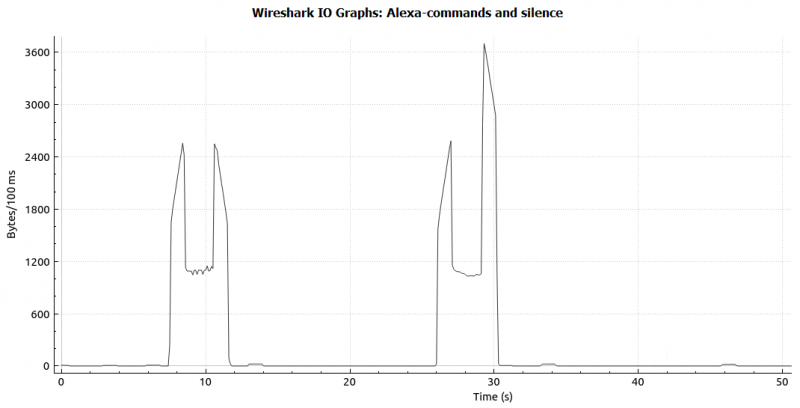
\includegraphics[width=5.00in,height=3.5in]{alexa_wakeup_and_pause-400x204.png}
\caption{Transmitted bytes in the given scenario}
\end{figure}
\end{itemize}

\subsection{Final solution}




\section{Business modelling and planning}
\label{sec:Business modelling and planning}
\subsection{Business modelling}
\subsection{Business planning}


\section{Business development process}
\label{sec:Business development process}

\section{Self evaluation}

\bibliography{II2202-report}
%%\bibliographystyle{IEEEtran}
\bibliographystyle{myIEEEtran}
%\appendix



\end{document}
